
\section{Preambulo}

\subsection{Nociones básicas de la combinatoria}

Cuando alguien se pregunta qué es la combinatoria, una respuesta típica es decir que se trata de ''el arte y la ciencia de contar''. Y es que, al contrario de lo que muchos intuitivamente podrían pensar, contar no es una actividad que siempre resulte ser trivial. En concreto, a la hora de realizar un conteo, nos vamos a enfrentar a dos dificultades elementales: contar todos los elementos y no repetir los elementos contados. Por lo que la combinatoria no solo se trata de ''contar'', sino de ''contar bien''.

Ahora, si bien los métodos de recuento forman parte esencial de la combinatoria, esta también contempla otros aspectos, entre ellos: el estudio de configuraciones conocidas, el estudio de la existencia de ciertas configuraciones, el conteo del número de configuraciones de un tipo dado, la enumeración o descripción de configuraciones, la optimización combinatoria, es decir, la determinación de las configuraciones que maximizan o minimizan una función dada, entre otras. En cualquier caso, el campo abierto a la combinatoria es amplio y fascinante, repleto de bellos resultados e interesantes problemas sin resolver.

En resumen, el conteo es una de las tareas básicas que se realizan en las matemáticas, he aquí su importancia. En este sentido, el objetivo de este curso será ser capaz de determinar cuantos elementos hay, sin caer en la necesidad de contarlos uno a uno.

\subsection{Ejercicios introductorios}

%\begin{ejercicio}
    %Hay tres caminos que van de la ciudad $A$ a la ciudad $B$, y cuatro caminos que van de la ciudad $B$ a la ciudad $C$. ¿De cuántas maneras podemos ir de la ciudad $A$ a la $C$ pasando por $B$? (No es válido regresarse).
%\end{ejercicio}

\begin{ejercicio}
    Hay tres caminos que van de la ciudad $A$ a la ciudad $B$, cuatro caminos que van de la ciudad $B$ a la ciudad $C$, y 5 caminos que van de la ciudad $A$ a la ciudad $C$. ¿De cuántas maneras podemos ir de la ciudad $A$ a la $C$? (No es válido regresarse).
\end{ejercicio}

\begin{ejercicio}
    Disponemos de tres cartas iguales, y de cinco sobres de diferentes colores: amarillo, blanco, café, dorado y escarlata. Vamos a guardar las cartas en los sobres, pero cada sobre puede contener a lo sumo una. ¿De cuántas maneras podemos guardar las cartas en los sobres?
\end{ejercicio}

\begin{ejercicio}
    El garaje de la casa de Ángela tiene cinco plazas. Con ella viven sus hermanas Beatriz y Carmen. Cada una tiene su propio coche, y cada día lo pueden colocar en el lugar que prefieran si no está ocupado. Este es el diagrama de la cochera:

    \begin{center}
        \begin{tabular}{|c|c|c|c|c|}
            1 & 2 & 3 & 4 & 5
        \end{tabular}
    \end{center}

    Por ejemplo, Ángela puede estacionar su coche en el lugar número 1, Beatriz en el número 2, y Carmen en el 4. ¿De cuántas maneras pueden Ángela, Beatriz y Carmen estacionar sus coches?
\end{ejercicio}

\begin{ejercicio}
    ¿Cuántas placas de vehículos distintas hay con dos letras a la izquierda y tres números a la derecha?
\end{ejercicio}

\begin{ejercicio}
    Tres estudiantes son enviados a un concurso de declamación. Desde luego, todos desean ser el primero en pasar. Supongamos que los estudiantes se llaman Ana, Benito y Carmen (los llamaremos A, B y C). Escriba todos los órdenes posibles en los que podrían pasar a declamar. Por ejemplo, si escribimos A B C , significa que pasarían en orden Ana, Benito y Carmen.
\end{ejercicio}

\begin{ejercicio}
    Manuel tiene cuatro carritos de juguete de diferentes colores (azul, blanco, verde y rojo, uno de cada color) y decide regalárselos a sus hermanos Luis y Karen. ¿De cuántas maneras diferentes puede hacer esto? Ejemplo: podría dar los cuatro carritos a Luis. También podría dar tres de ellos a Karen y el otro a Luis.
\end{ejercicio}

\begin{ejercicio}
    En una fiesta, cuatro amigos se van a dar regalos entre sí, de manera que cada uno dé un regalo y reciba otro. Desde luego, nadie debe darse el regalo a sí mismo (algo así como jugar amigo secreto). ¿De cuántas formas es posible hacer la distribución?
\end{ejercicio}

\section{Conjuntos}

\subsection{Nociones básicas de los conjuntos}

\begin{definicion}
    Con el término \textbf{conjunto} nos referimos a ''una colección bien definida de elementos dentro de un todo, considerada en sí misma como un objeto''. El concepto ''bien definido'' significa que para un objeto dado es posible determinar si pertenece o no al conjunto. Los elementos de un conjunto pueden ser casi cualquier cosa: números, personas, letras, etc. Pueden ser incluso otros conjuntos. De forma específica, en matemáticas existen varios conjuntos de números que son especialmente importantes: el conjunto de los números naturales ($\mathbb{N}$), el de los números enteros ($\mathbb{Z}$), el de los números racionales ($\mathbb{Q}$) y el de los números reales ($\mathbb{R}$).
\end{definicion}

Para representar, por ejemplo, que $S$ es el conjunto que contiene los elementos $a, b$ y $c$, escribimos

\begin{center}
    $S=\{a,b,c\}$.
\end{center}

Para indicar que $a$ es un elemento del conjunto $S$, escribimos $a \in S$, y se lee ''$a$ pertenece a $S$''. Generalmente, para nombrar un conjunto, se utilizan letras mayúsculas.

Para definir un conjunto, se puede simplemente elegir o listar cuáles son los elementos que lo componen (\textbf{definición por extensión}). También se puede definir un conjunto enunciando una propiedad que permita determinar si un objeto pertenece al conjunto o no (\textbf{definición por compresión}). En general, un conjunto puede definirse de dos formas:  por extensión y por comprensión.

Por ejemplo, si deseamos expresar que $A$ es el conjunto de los números pares positivos, por extensión tenemos

\begin{center}
    $A=\{2,4,6,8,...\}$
\end{center}

y por comprensión tenemos $$A=\{El \ conjunto \ de \ los \ n\Acute{u}meros \ pares \ positivos\}.$$ O expresado en términos más formales

\begin{center}
    $A=\{2n \ | \ n \in \mathbb{N} \}$
\end{center}

y se lee como ''$A$ es el conjunto de los números de la forma $2n$ tal que $n$ pertenece a los números naturales''. Los símbolos ''$|$'' y ''$:$'' se pueden leer como ''tal que''.

\subsection{Conceptos importantes}

\textbf{Pertenencia:} Dado que los conjuntos son colecciones de objetos, es necesario tener una simbología para indicar que un elemento forma parte del conjunto; escribimos $a\in A$ para indicar que $a$ es un elemento de $A$ y $a \notin A$ significa que $a$ no es un elemento del conjunto $A$.   

\textbf{Conjunto Vacío:} El conjunto que no tiene  elementos se denomina conjunto vacío, y se representa con el símbolo $\varnothing$, o escribiendo dos llaves: $\{\}$, cabe recalcar que el conjunto vacío es único.

\textbf{Cardinalidad:} A la cantidad de elementos que posee un conjunto se le conoce como la cardinalidad del conjunto, y se denota como $|S|$ donde $S$ es algún conjunto dado. Por ejemplo, si se tiene un conjunto $A=\{a, b, c, d, e\}$ entonces $|A|= 5$. La cardinalidad de un conjunto puede ser infinita, como en el caso de los números naturales, o cero, en el caso del conjunto vacío.

\textbf{Igualdad de Conjuntos:} Dos conjuntos son iguales si y solamente si, poseen los mismos elementos.

\textbf{Ejemplo.} El conjunto de números naturales es igual al conjunto de los enteros positivos, o dicho de otra manera: $$\mathbb{N}=\mathbb{Z}^+$$

\textbf{Subconjuntos:} Si un conjunto $A$ cumple que todos sus elementos también son elementos de otro conjunto $B$, se dice que $A$ es un subconjunto de $B$, o que $A$ está incluido en $B$. Se escribe como $A \subset B$.  Por ejemplo, el conjunto de los números naturales es un subconjunto de los números enteros, es decir, $\mathbb{N} \subset \mathbb{Z}$. Además, todo conjunto es subconjunto de sí mismo ($A\subset A$) y además el conjunto vacío es un subconjunto de cualquier otro conjunto ($\emptyset \subset A$).

\textbf{Conjunto Potencia:} Dado un conjunto $A$, se le denomina conjunto potencia de $A$, al conjunto cuyos elementos son todos los subconjuntos de $A$ y se denota por $\mathcal{P}(A)$. Por ejemplo, si $A=\{a,b\}$, entonces $\mathcal{P}(A)=\{\varnothing,\{a\},\{b\},\{a,b\}\}$. Notemos que $\emptyset \in \mathcal{P}(A)$ y $\emptyset \subset \mathcal{P}(A)$.

\subsection{Operaciones con conjuntos}

Los conjuntos pueden ser representados mediante digramas de Venn, en los diagramas de Venn el conjunto universal $\mathbb{U}$ que contiene todos los objetos bajo consideranción está representado por un rectángulo, dentro de esto se utilizan círculos u otras figuras geométricas para representar a los conjuntos. En la siguiente figura tenemos una representación general para tres conjuntos $A, B$ y $C$.

\begin{center}
    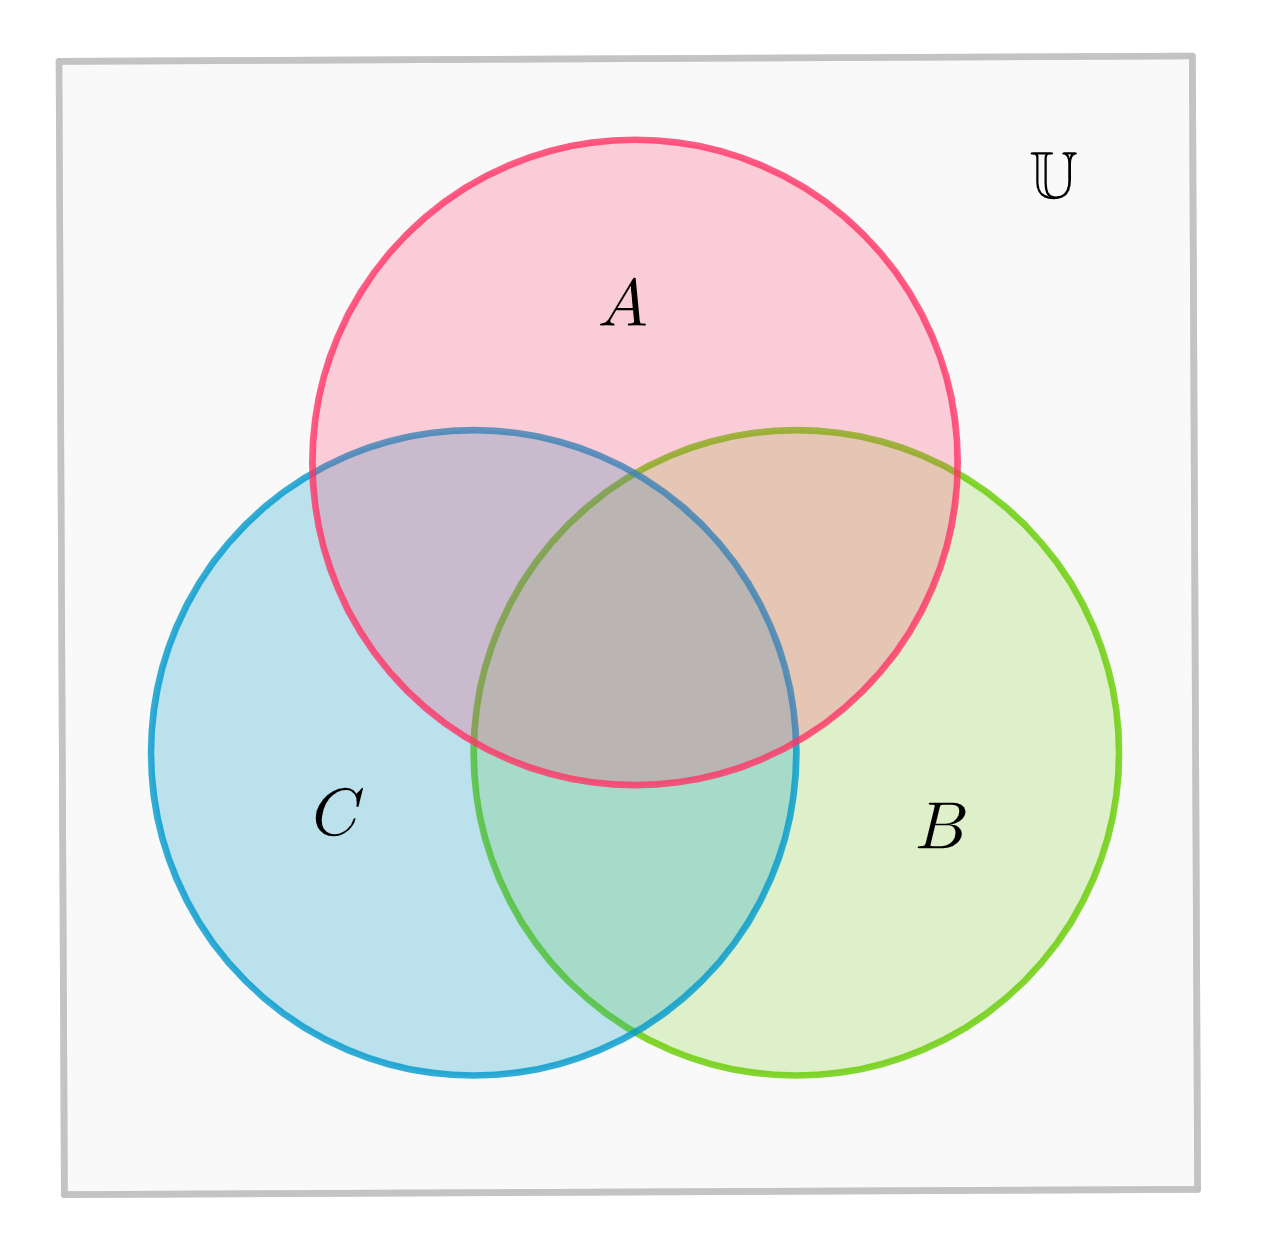
\includegraphics[scale=0.7]{Imagenes/IMG1/S1-1-01.png}
\end{center}

\textbf{Unión de conjuntos:} Sean $A$ y $B$ dos conjuntos. Entonces, el conjunto unión de $A$ con $B$ se denota por $A \cup B$, y está formado por todos los elementos que pertenecen al conjunto $A$, al conjunto $B$, o a ambos. El color rosa de la figura adjunta representa la el conjunto unión de $A$ y $B$.

\begin{center}
    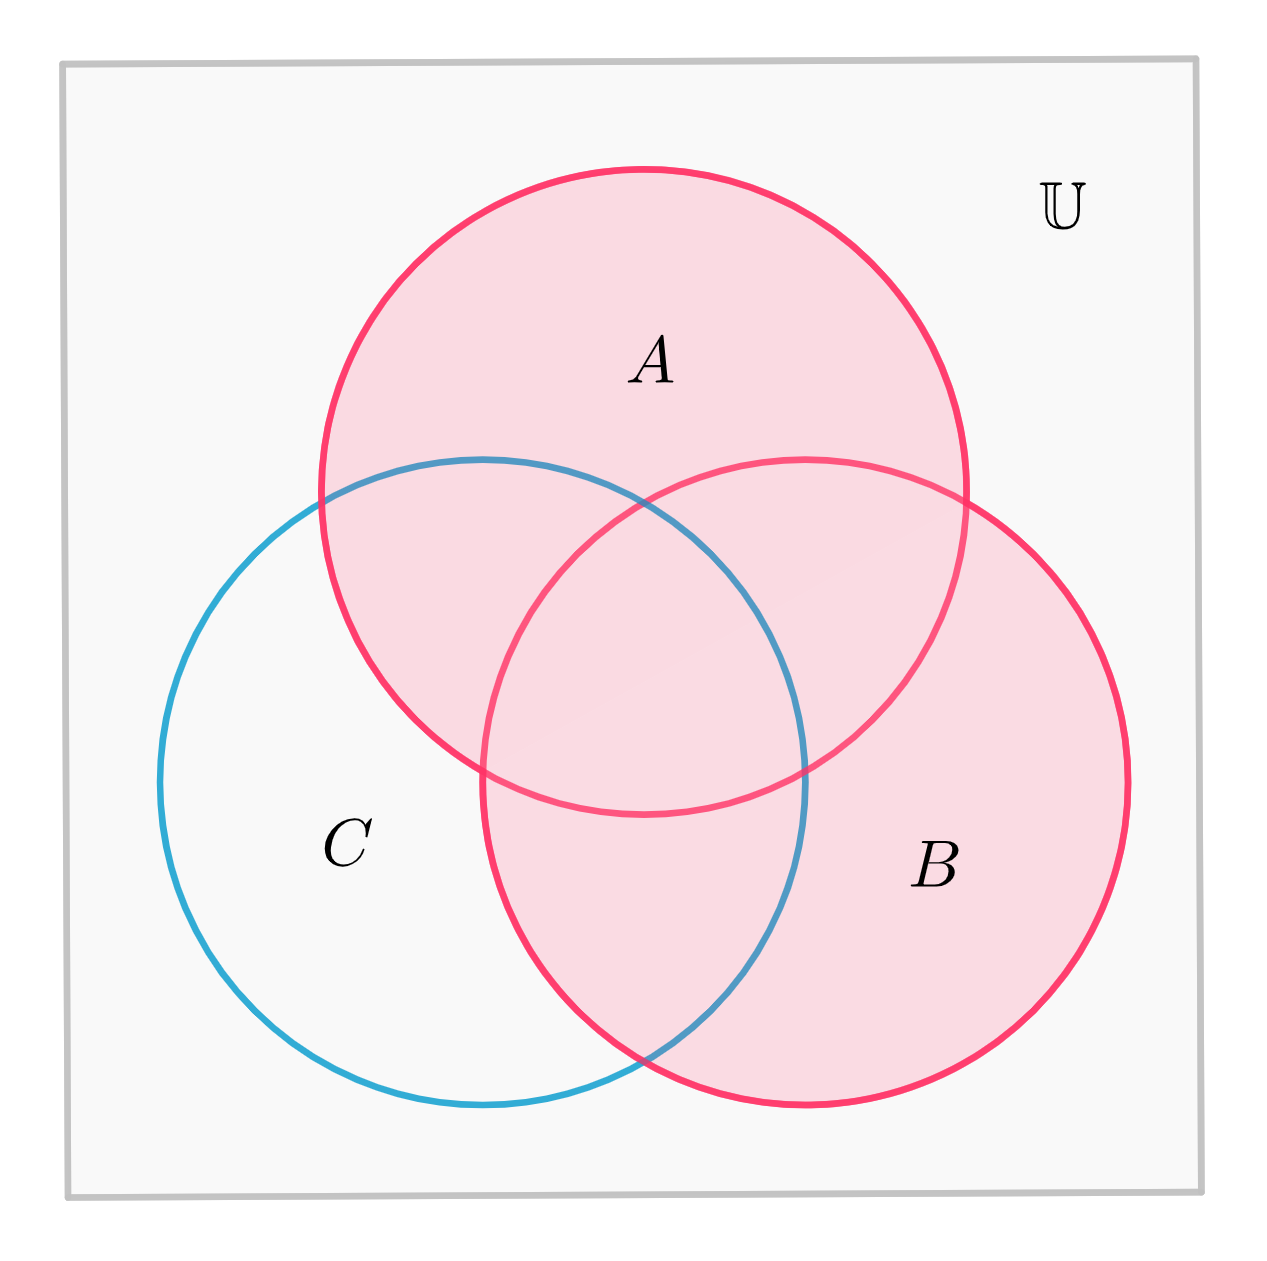
\includegraphics[scale=0.7]{Imagenes/IMG1/S1-1-02.png}
\end{center}

En la figura anterior la intersección de $A$ y $B$ es la parte de color morado.

\begin{ejemplo}
    Sea $A=\{x \ | \ x \in \mathbb{N}, \ 10 \leq x < 14\}$ y $B=\{y \ | \ y \ es \ par, \ 6<y<18\}$. Encontrar $A \cup B$.
\end{ejemplo}

\begin{solucion}
    Se deben definir los conjuntos por extensión, por lo que $A=\{10,11,12,13\}$ y $B=\{8,10,12,14,16\}$.  Entonces, $A \cup B=\{8,10,11,12,13,14,16\}$.
\end{solucion}

\textbf{Intersección de conjuntos:} Sean $A$ y $B$ dos conjuntos. Entonces, el conjunto intersección de $A$ y $B$ se denota por $A \cap B$, y está formado solo por los elementos que pertenecen a ambos conjuntos. 

\begin{center}
    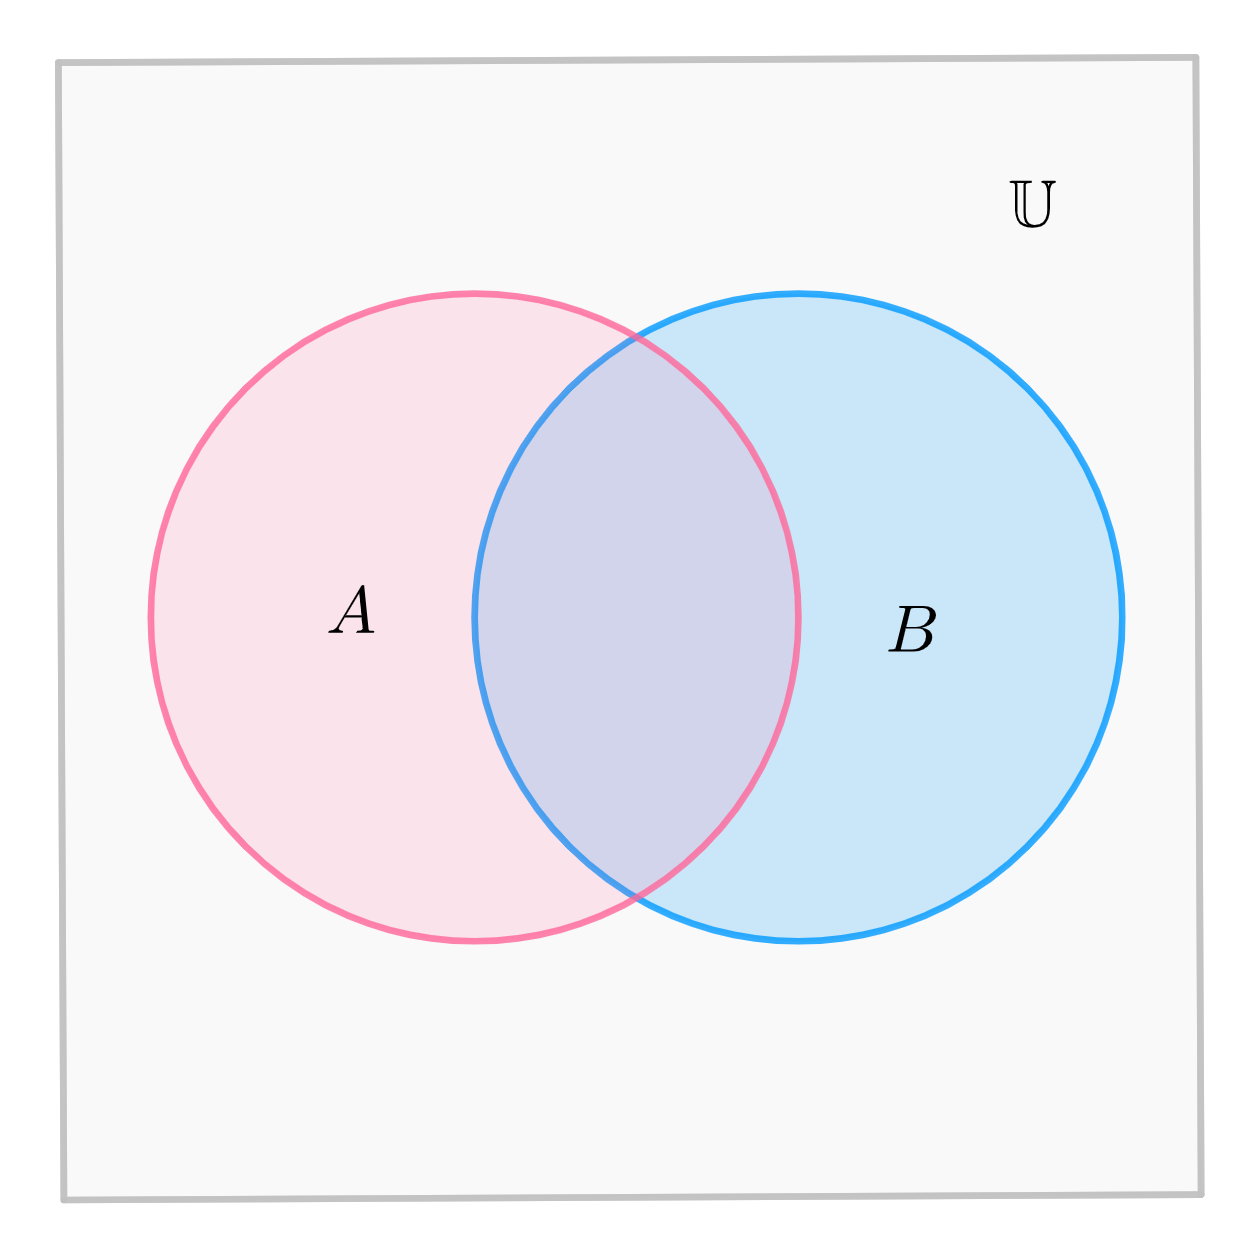
\includegraphics[scale=0.7]{Imagenes/IMG1/S1-1-03.png}
\end{center}

\begin{ejemplo}
    Si $A=\{\text{\textbf{las vocales}}\}$ y $B=\{x \ | \,\text{$x$ es una letra de la palabra}\;\text{\textbf{combinatoria}}\}$, hallar $A \cap B$.
\end{ejemplo}

\begin{solucion}
    Al definir los conjuntos por extensión, tenemos que $A=\{a,e,i,o,u\}$ y, eliminando las repreticiones, $B=\{c,o,m,b,i,n,a,t,r\}$.  Por lo tanto, los elementos en común son $A \cap B=\{a,i,o\}$.
\end{solucion}

\textbf{Diferencia de conjuntos:} Sean $A$ y $B$ dos conjuntos. Entonces, se denota por $A-B$ al conjunto formado por todos los elementos de $A$ que no pertenecen a $B$. De cierta forma significa ''quitarle a $A$ todos los elementos que también pertenecen a $B$''.

\begin{ejemplo}
    Si se tiene que $A=\{-5,1,-3,2,-2,9\}$ y $B=\{x \ | \ x \in \mathbb{N} \}$, ¿cuáles son los elementos de $A-B$?
\end{ejemplo}

\begin{solucion}
    El conjunto $A$ ya esta difinido por extensión y $B$ es el conjunto de los números naturales.  Al quitarle a $A$ todos los elementos que también pertenecen a $B$, nos resulta $A-B=\{-5,-3,-2\}$.
\end{solucion}

\textbf{Complemento de un conjunto:} Sea $A$ un subconjunto del conjunto universal $\mathbb{U}$. Entonces el conjunto complemento de $A$ relativo al conjunto $\mathbb{U}$, se denota por $A'$ o por $A^c$, y está compuesto por todos los elementos de $\mathbb{U}$ que no pertenecen a $A$, en notación de conjuntos $A'=\mathbb{U}-A$. En la siguiente figura el sector de color gris representa el complemento del conjunto $B$.

\begin{center}
    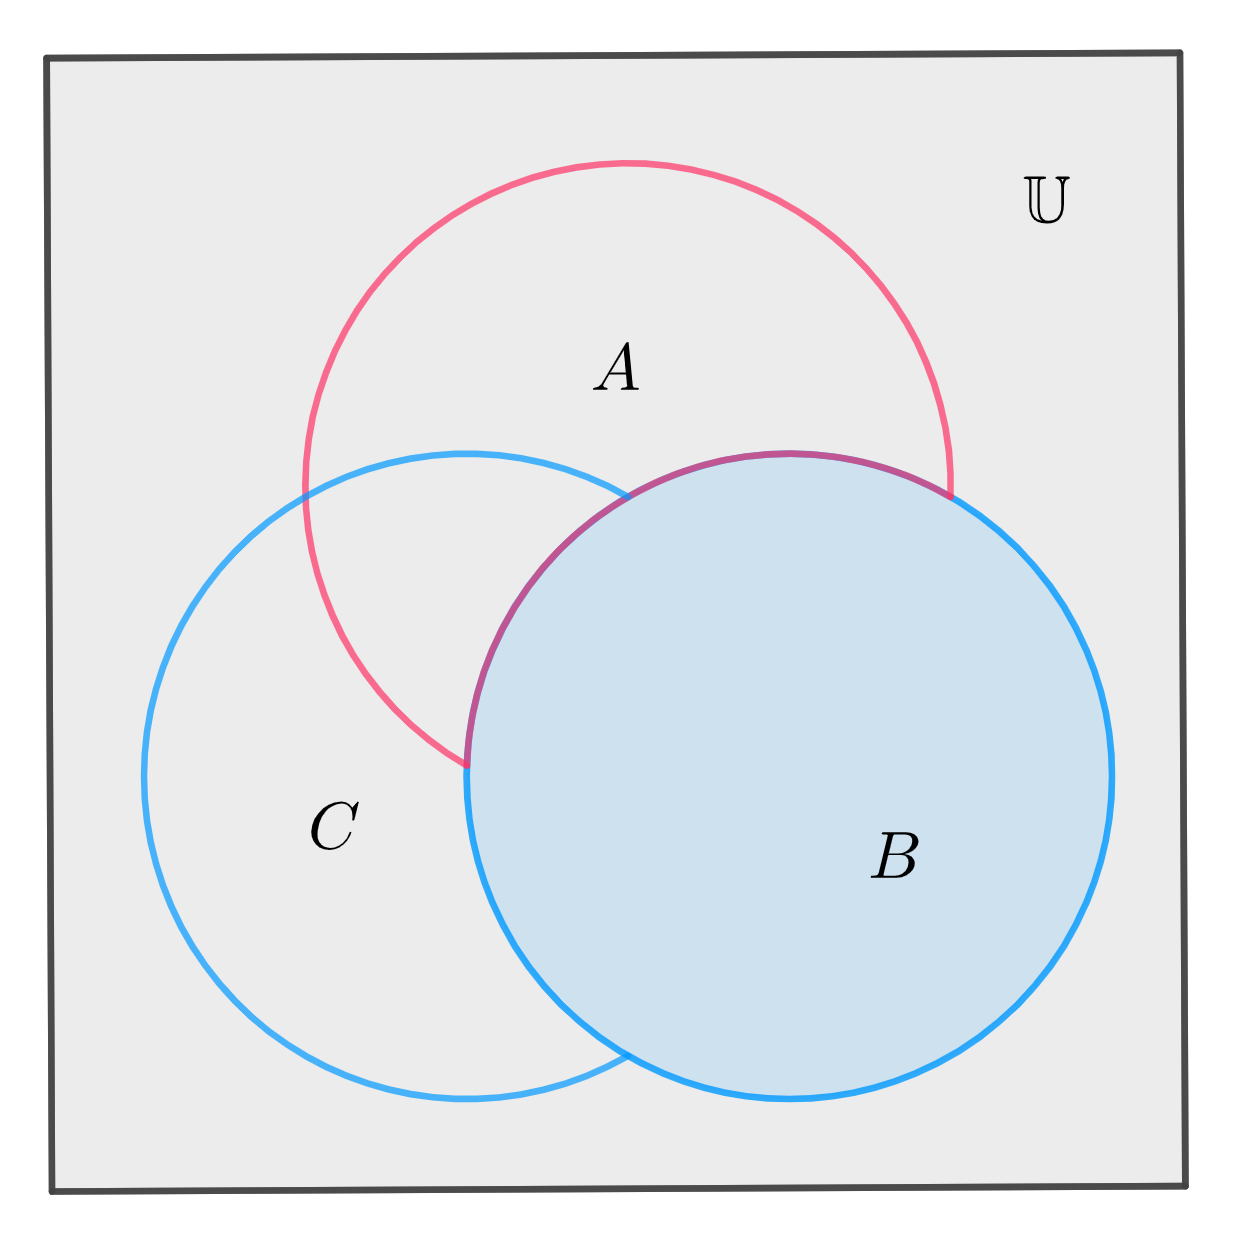
\includegraphics[scale=0.7]{Imagenes/IMG1/S1-1-05.png}
\end{center}

\begin{ejemplo}
    Si $A$ es el conjunto de los números enteros positivos ($\mathbb{Z}^{+}$) En el universo $\mathbb{U}$ de los números enteros ($\mathbb{Z}$). ¿Quién es $A'$?
\end{ejemplo}

\begin{solucion}
    Bajo la idea de complemento se puede hacer la iguiente pregunta:  ¿qué le hace falta a $\mathbb{Z}^{+}$ para ser el conjunto de los $\mathbb{Z}$?.  Al responder la pregunta, nos damos cuenta de que $A'=\mathbb{Z}^{-}_{0}$.
\end{solucion}

\begin{ejemplo}
    Si se tienen los conjuntos:

    \begin{center}
        $A =\{0, 1, 2, 7, 8\}$ \\
        $B =\{1, 3, 4, 5, 8\}$ \\
        $\mathbb{U} =\{0, 1, 2, 3, 4, 5, 6, 7, 8, 9\}$
    \end{center}

    Determinar $A \cup B$, $A \cap B$, $A-B$ y $A'$. Además, determinar $|A|$, $|B|$, $|A \cap B|$ y $|A \cup B|$. ¿Nota alguna relación entre estas cardinalidades?
    
\end{ejemplo}

\begin{solucion} Los resultados de las operaciones serían

    \begin{center}
        $A \cup B=\{0,1,2,3,4,5,7,8\}$ \\
        $A \cap B=\{1,8\}$ \\
        $A-B=\{0,2,7\}$ \\
        $A'=\{3,4,5,6,9\}$ \\
        $|A|=5$, $|B|=5$, $|A \cap B|=2$ y $|A \cup B|=8$
    \end{center}

    Notar que, para cualesquiera par de conjuntos, se cumple que $|A \cup B| = |A| + |B| - |A \cap B|$.
    
\end{solucion}

\section{Principios fundamentales en el conteo}
Imagínate por un momento que vas de compras en algún día tranquilo de la semana. Seleccionas un buen par de jeans y decides pagar con tu tarjeta de crédito (o con la de sus padres). Pero de repente te das cuenta de que no puedes recordar tu pin. ¡Qué tragedia! Ahora todo lo que se te ocurre es hacer una lista de todas las combinaciones posibles para descubrir tu pin. \textit{¿Cuántas combinaciones posibles puedes hacer?} La respuesta a esta pregunta es \textit{difícil} si seguimos enumerando cada combinación posible y contando. En situaciones como estas, el principio fundamental del conteo o el principio de multiplicación viene a nuestro rescate. Y en otras situaciones con más restricciones es pertinente usar el conocido principio de la suma. %En esta lección vamos a estudiar ambos resultados y haremos hincapié en las aplicaciones así como en su diferenciación.
\subsection{Principio de la multiplicación}
\begin{definicion}
    El principio fundamental de conteo o principio de la multiplicación es una regla que se usa para contar el número total de resultados posibles en una situación de dos eventos consecutivos. El principio de la multiplicación establece que si una actividad puede realizarse de $n$ formas distintas y, para cada una de esas formas, una segunda actividad puede realizarse de $m$ maneras distintas, entonces las dos actividades consecutivas pueden realizarse de $nm$ maneras diferentes. 
\end{definicion}

\begin{ejemplo}
    ¿De cuántas maneras se pueden elegir un presidente y un vicepresidente de $25$ candidatos?
\end{ejemplo}

\begin{solucion}
De los $25$ candidatos, hay $25$ formas posibles de elegir un presidente. Después de elegir al presidente, quedan $24$ candidatos para elegir un vicepresidente. Por el principio de la multiplicación tenemos entonces que hay
\[25\times 24=600\]
maneras de elegir al presidente y al vicepresidente.
\end{solucion}

\begin{ejemplo}
    Erick fue a la tienda después de la escuela para recoger una jarra de leche, una barra de pan, una docena de huevos y un paquete de galletas. La leche viene en variedades de $1\%$, $2\%$ y $3,25\%$. El pan viene en blanco y $100\%$ integral. Los huevos vienen en paquetes de docenas de varios tamaños: pequeños, medianos, grandes y jumbo. Las galletas vienen en tres sabores diferentes. ¿De cuántas maneras diferentes puede Erick llevar a casa los elementos de su lista?
\end{ejemplo}

\begin{solucion}
Usamos la propiedad de multiplicación de contar, ya que Erick está comprando uno de cada artículo. Tiene $3$ opciones de leche, $2$ de pan, $4$ de huevos y $3$ de galletas, así que tiene $3\times 2 \times 4 \times 3=72$ diferentes maneras de llevar a casa los elementos de su lista.
\end{solucion}

\begin{ejemplo}
    Para ir de la ciudad $A$ a la ciudad $D$ debemos de pasar por la ciudad $B$ y $C$ respectivamente.

    \begin{center}
        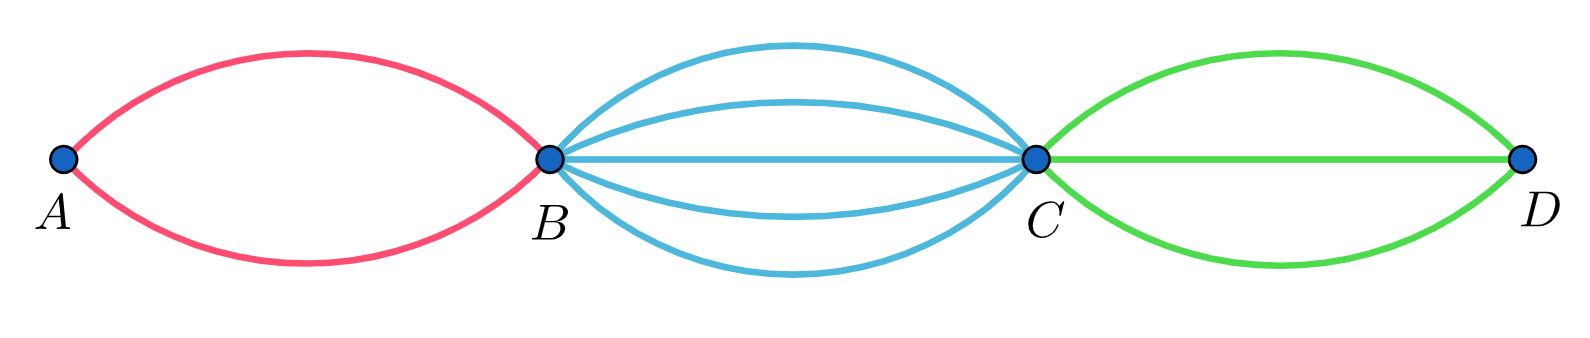
\includegraphics[scale=0.3]{Imagenes/IMG1/S1-1-07.png}
    \end{center}

    Tenemos dos rutas para ir de la ciudad $A$ a la ciudad $B$, cinco rutas para ir de la ciudad $B$ a la ciudad $C$ y tres rutas para ir de la ciudad $C$ a la ciudad $D$. Por lo tanto tenemos $2 \times 5 \times 3=30$ rutas distintas para ir de la ciudad $A$ a la ciudad $D$.
\end{ejemplo}

\begin{solucion}
    
\end{solucion}

\begin{ejemplo}
    En el armario de Brenda hay $4$ pantalones diferentes, $9$ camisas diferentes y $n$ chaquetas diferentes. Si la cantidad de combinaciones de pantalones, camisas y chaquetas que Brenda puede elegir es $252$, ¿cuántas chaquetas diferentes tiene?
\end{ejemplo}

\begin{solucion}
    Para cada una de las $n$ chaquetas diferentes, hay $4$ pantalones diferentes y $9$ camisas diferentes para elegir. Así, el número total de combinaciones es de $4\times 9 \times n$ y lo cual
    \begin{eqnarray*}
        4\times 9 \times n&=&252\\
        n&=&7
    \end{eqnarray*}
    Así, Brenda tiene $7$ chaquetas diferentes.
\end{solucion}

\begin{ejemplo}
    ¿Cuántos divisores positivos tiene $2024$?
\end{ejemplo}

\begin{solucion}
    Notemos que $2024=2^3\cdot 11 \cdot 23$, entonces cualquier divisor del número $2024$ debe tener la forma $2^k\times 11^m \times 23^n$, donde $0\leq k\leq 3$, $0\leq m\leq 1$ y $0\leq n\leq 1$. En consecuencia, hay $4$ posibilidades para $k$, $2$ posibilidades para $m$ y también $2$ posibilidades para $n$. Por tanto, hay
    \[4\times 2 \times 2=16\]
    divisores positivos de $2024$ en total.
\end{solucion}

\begin{ejemplo}
Si cuenta las formas de subir 3 escalones encontrará que hay 4 formas de subir 3 escalones. Imagine que las piernas de la persona son tan largas que tiene la capacidad de subir 11 escalones a la vez. Además, a la persona solo se le permite subir hacia arriba. Encontrar el número de formas en que puedes subir 11 escalones. \textbf{Bonificación}: Generalice esto para $n$ pasos.
\end{ejemplo}

\begin{solucion}
Aquí, hay $11$ escalones. Ahora, pisar cualquiera de los primeros $10$ escalones no es obligatorio, pero es obligatorio para el $11^\circ$ Escalón, porque es donde tenemos que subir. Entonces, hay $2$ opciones para los primeros $10$ escalones, pero solo $1$ para el $1$. Por lo tanto, según la regla del producto, el número de formas de subir a la escalera $11$ es:
\[2\times 2\times 2\times 2\times 2\times 2\times 2\times 2\times 2\times 2\times 1=2^{10}=1024\;. \]
La persona tiene que subir el escalón $n$-ésimo obligatoriamente. Pero la persona en los primeros $n-1$ escalones lo pisa o no lo pisa. Por lo tanto, hay $2$ posibilidades para cada paso de los $n-1$ escalones. Entonces, por regla de la multiplicación, el total de formas es \[\underbrace{2\times 2 \ldots \times 2}_{n-1\;\text{veces}}\times 1=2^{n-1}\]
y si $n=11$, nuestra resolución es consistente.
\end{solucion}

\begin{ejemplo}
¿Cuántos números capicuas existen de $5$ cifras tales que el producto de sus cifras sea un cuadrado perfecto?
\end{ejemplo}

\begin{solucion}
Sea el número capicua $\displaystyle \overline{xyzyz}$. Para que el producto de las $5$ cifras sea un cuadrado perfecto, debemos analizar los posibles valores de $z$.
\[x^2\times y^2\times z:=\text{algún cuadrado perfecto}\]
De hecho para que esto se satisfaga $z$ puede ser $1$, $4$ y $9$, es decir, $z$ debe ser un cuadrado perfecto. Ahora vemos que $z$ toma $3$ posibles valores. Luego, podemos asignar a $x$ nueve posibles valores (¿por qué?) y a $y$ diez posibles valores. Por tanto, por el principio de la multiplicación tenemos que:
\[9\times 10 \times 3=270\]
es el total de números capicuas deseados.
\end{solucion}

\begin{ejemplo}
    Si $M$ es el número de palíndromos de $3$ dígitos y $N$ es el número de palíndromos de $4$ dígitos, ¿cuál es mayor? ¿o son iguales?
\end{ejemplo}
\begin{solucion}
Primero calculemos $M$, el número de palíndromos de $3$ dígitos. Imagine construir un palíndromo de $3$ dígitos eligiendo los dígitos secuencialmente, comenzando desde la izquierda. Hay $9$ opciones para el primer dígito (más a la izquierda), ya que puede ser cualquier dígito que no sea $0$. Después de elegir el primer dígito, hay $10$ opciones para el segundo dígito (independientemente de la elección para el primer dígito). Para que el número sea un palíndromo, el último dígito debe ser el mismo que el primero, por lo que después de elegir el primer dígito, solo hay $1$ opción para el último dígito. El número total de formas de elegir los dígitos es el producto de estos números:
\[M=9\times 10\times 1=90\]
Ahora calculemos $N$, el número de palíndromos de $4$ dígitos. Nuevamente, imagine construir un palíndromo de $4$ dígitos eligiendo los dígitos secuencialmente, comenzando desde la izquierda. Hay $9$ opciones para el primer dígito (más a la izquierda), ya que puede ser cualquier dígito que no sea $0$. Después de elegir el primer dígito, hay $10$ opciones para el segundo dígito (independientemente de la elección para el primer dígito). Para que el número sea un palíndromo, el tercer dígito debe ser el mismo que el segundo dígito y el último dígito debe ser el mismo que el primer dígito, por lo que después de elegir el primer y el segundo dígito, solo hay $1$ opción para el tercer dígito y $1$ opción para el último dígito. El número total de formas de elegir los dígitos es el producto de estos números:
\[N=9\times 10 \times 1 \times 1=90\]
Así tenemos que $M=N$.
\end{solucion}

\subsection{Principio de la suma}
\begin{definicion}
El principio de la suma es un enfoque de conteo básico en combinatoria. Una declaración básica del principio es que si un evento $A$ puede ocurrir de $n$ opciones  y un suceso $B$ puede ocurrir de $m$ maneras, y ambos sucesos no pueden ocurrir simultaneamente, entonces hay $n+m$ formas de que ocurra alguno de los eventos. .
\end{definicion}

\begin{obs}
El principio de la suma solo se aplica a las opciones que son \textit{mutuamente excluyentes}, lo que significa que solo se puede elegir una de las opciones. Para determinar cuándo usar el principio de la suma (en oposición al principio de la multiplicación), intente reformular la pregunta. Si la pregunta se puede reformular con la palabra ''o", esto generalmente indica que se aplica el principio de la suma.
\end{obs}

El principio de la suma se puede también enunciar utilizando conjuntos; en efecto si un dos conjuntos finitos $A$ y $B$ no tienen elementos en común ($A\cap B=\emptyset$), entonces $$|A\cup B|=|A|+|B|.$$ 

\begin{multicols}{2}
\,\
\begin{ejemplo}

 Supongamos que queremos ir de la ciudad $P$ a la ciudad $Q$, para ello tenemos dos rutas por aire, dos rutas por el oceano y tres rutas para ir por vía terrestre, por lo tanto el total de rutas para ir de $P$ a $Q$ tenemos $2+3+3=7$.
 \,\\
 \,\\

\begin{center}
    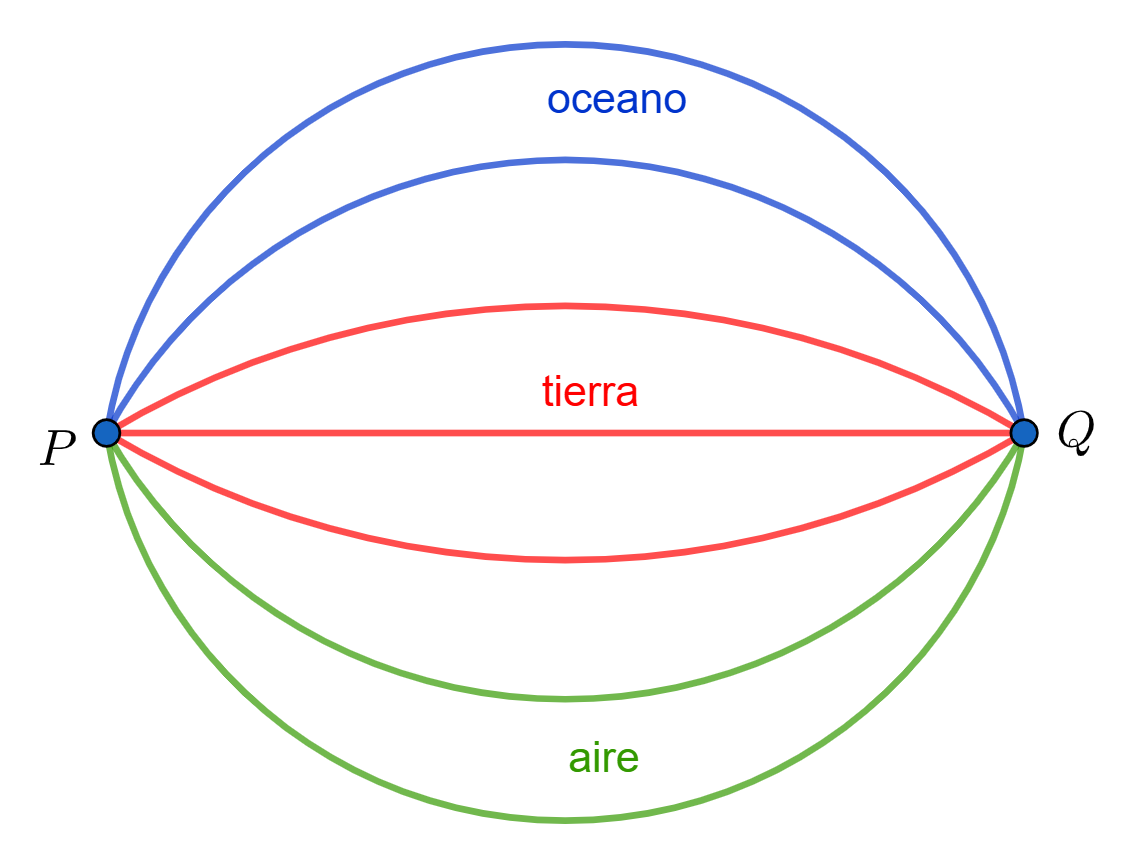
\includegraphics[scale=0.3]{Imagenes/IMG1/S1-1-06.png}
\end{center}       
\end{ejemplo}
\end{multicols}

\begin{ejemplo}
Probar que $|A \cup B|=|A|+|B|-|A\cap B|$.
\end{ejemplo}

\begin{solucion}
Notemos que $A \cup B = (A-B)\cup B$, y además $(A-B) \cap B = \emptyset$, luego $$|A\cup B|=|A-B|+|B|.$$ Por otro lado tenemos que $A= (A-B)\cup (A\cap B) $ donde también $(A-B)\cap (A\cap B)=\emptyset$, aplicando el principio de la suma tenemos que $$|A|=|A-B|+|A\cap B|.$$

Luego tenemos 
\begin{eqnarray*}
|A\cup B| & = &  |A-B|+|B|\\
&=& |A|-|A\cap B|+|B|
\end{eqnarray*}
obteniendo la fórmula deseada.
\end{solucion}

\begin{ejemplo}
Sea $X$ el conjunto de los enteros consecutivos $\left\{16,17,\ldots,51\right\}$ y sea $Y$ el conjunto de los enteros consecutivos $\left\{70,71,\ldots,111\right\}$. ¿Cuántos enteros diferentes hay en $X$ o $Y$?
\end{ejemplo}
\begin{solucion}
Para el conjunto $X$ tenemos que $|X|=51-16+1$ números y en el conjunto $Y$ tenemos. también, que $|Y|=111-70+1=42$ números. Dado que no hay superposición entre los dos conjuntos, según el principio de la suma, hay $36 + 42 = 78$ números en $X$ o $Y$.
\end{solucion}

\begin{ejemplo}
¿Cuántos palíndromos de $3$ dígitos hay donde el dígito medio es más grande que los dígitos exteriores (como $121$)?
\end{ejemplo}

\begin{solucion}
Imaginemos que construimos un palíndromo de $3$ dígitos donde el dígito del medio es más grande que los dígitos exteriores eligiendo los dígitos secuencialmente, comenzando desde la izquierda. Si el primer dígito (más a la izquierda) es un $1$, entonces hay $8$ opciones ($2$ a $9$) para el segundo dígito y $1$ opción para el último dígito; si el primer dígito es un $2$, entonces hay $7$ opciones ($3$ a $9$) para el segundo dígito y $1$ opción para el último dígito; y así sucesivamente, hasta que, finalmente, si el primer dígito es un $9$, entonces hay $0$ opciones para el segundo dígito (ya que ningún dígito es mayor que $9$). El número total de formas de elegir los dígitos es la suma de estos números:
\[8+7+6+5+4+3+2+1+0=36\;.\]
\end{solucion}

\begin{ejemplo}
¿Cuántos triángulos puedes hallar en la siguiente figura?
\begin{figure}[h]
    \centering
    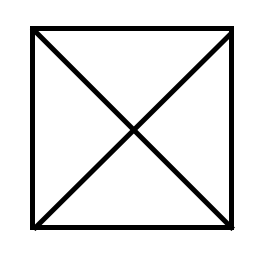
\includegraphics[scale=0.5]{Imagenes/IMG1/square.png}
\end{figure}
\end{ejemplo}
\begin{solucion}
Claramente hay 4 triángulos pequeños y cuatro triángulos grandes que se forman uniendo dos triángulos pequeños, por lo que son 8 triángulos en total. Es decir,
\[\underbrace{4}_{\text{triángulos pequeños}}+\underbrace{4}_{\text{triángulos grandes}}=8\;.\]
\end{solucion}

\begin{ejemplo}
¿cuántos cuadrados puedes encontrar en la figura \ref{cuadrado}?
\begin{figure}[h]
    \centering
    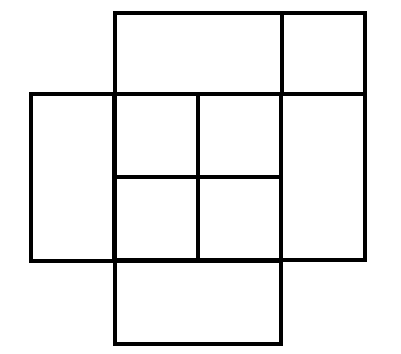
\includegraphics[scale=0.5]{Imagenes/IMG1/fig.png}
    \caption{¿Podrías identificar la cantidad de cuadrados?}
    \label{cuadrado}
\end{figure}
\end{ejemplo}

\begin{solucion}
Comencemos contando los cuadrados más grandes que son $1$, el cuadrado de $3\times 3$, luego cuente los cuadrados de $2\times 2$, que son $5$, luego los cuadrados de $1\times 1$ que son $5$. 
\begin{itemize}
    \item $3\times 3$: $1$ cuadrado;
    \item $2\times 2$: $5$ cuadrados;
    \item $1\times 1$: $5$ cuadrados
\end{itemize}
Luego el total de cuadrados es
\[1+5+5=11\;.\]
\end{solucion}



\section{Problemas propuestos}
\begin{problema}
    Encuentre la unión e intersección de los siguientes conjuntos.
    \begin{multicols}{2}
    \renewcommand{\labelenumi}{\alph{enumi})}
    \begin{enumerate}
        \item $\{3,4,5,6,7\}$ y $\{4,6,8,10\}$
        \item $\{9,14,25,30\}$ y $\{10,17,19,38,52\}$
        \item $\{a,b,d,f,g,h\}$ y $\{c,f,g,h,k\}$
        \item $\{3,4,5\}$ y $\varnothing$
    \end{enumerate}   
    \end{multicols}    
\end{problema}

\begin{problema}
    Sea $U=\{1,2,3,4,5,6,9\}$, $A=\{1,2,3,4\}$, $B=\{2,4,6\}$ y $C=\{3,5,7\}$. Encuentre y grafique en diagramas de Venn:
    \begin{multicols}{2}
    \renewcommand{\labelenumi}{\alph{enumi})}
    \begin{enumerate}
        \item $A' \cap B$
        \item $B' \cup C'$
        \item $A \cap (B \cup C')$
        \item $(A' \cup C') \cap (B')$
        
    \end{enumerate}    
    \end{multicols}   
\end{problema}

\begin{problema}
    Sea $U=\{1,2,3,4,5,6,7\}$, $A=\{1,2,3,4,5,6\}$, $B=\{2,3,6\}$ y $C=\{3,5,7\}$. Encuentre:
    \begin{multicols}{2}
    \renewcommand{\labelenumi}{\alph{enumi})}
    \begin{enumerate}
        \item $A-B$
        \item $B-A$
        \item $(A-B) \cup C)$
        \item $A'\cup B'$
        \item $B' \cap C'$
        \item $A \cap B \cap C$
    \end{enumerate}   
    \end{multicols}   
\end{problema}

\begin{problema}
    Suponga que se tienen dos conjuntos $A$ y $B$. Sombree en un diagrama de Venn las regiones que hacen referencia a las siguientes operaciones:
   \begin{multicols}{2}
        \renewcommand{\labelenumi}{\alph{enumi})}
    \begin{enumerate}
        \item $(A \cap B)'$
        \item $A' \cup B'$
        \item $(A \cup B)'$
        \item $A' \cap B'$
    \end{enumerate}
   \end{multicols}
    A estas propiedades se les conoce como \textbf{leyes de De Morgan}.
\end{problema}

\begin{problema}
Escribir el cardinal de cada uno de los siguientes conjuntos.
\begin{multicols}{2}
\renewcommand{\labelenumi}{\alph{enumi})}
    \begin{enumerate}
        \item $\{\emptyset, \{\emptyset\}, \{\emptyset, \{\emptyset\}\}\}$
        \item $\mathcal{P}(\mathcal{P}(\emptyset))$
    \end{enumerate}   
\end{multicols}
\end{problema}

\begin{problema}
¿Cuántos grupos diferentes integrados por un hombre y una mujer pueden formarse con $5$ hombres y $8$ mujeres, si cierto varón se rehusa a formar pareja con dos mujeres en particular?    
\end{problema}

\begin{problema}
En un tablero de $5\times 5$, ¿de cuántas maneras posibles se pueden colocar dos fichas sin que estén ni en la misma fila ni en la misma columna?
\end{problema}

\begin{problema}
Marisol tiene un dado estándar de $6$ caras y una moneda.  ¿Cuántos resultados diferentes puede obtener tirando el dado o lanzando la moneda?
\end{problema}

\begin{problema}
    Hay $8$ tarjetas con el número $10$, $5$ tarjetas con el número $100$ y $2$ tarjetas con el número $500$. ¿Cuántas sumas distintas son posibles usando de $1$ a todas las $15$ tarjetas?
\end{problema}

\begin{problema}
    ¿Cuántos números enteros positivos de $4$ dígitos tienen $2$ o más ceros?
\end{problema}

\begin{problema}
¿Cuántos números de tres cifras pueden escribirse de manera que la primera cifra sea impar, la segunda sea par y la tercera sea diferente de las dos primeras?
\end{problema}

\begin{problema}
    De un grupo de 5 estudiantes quiere elegirse una comisión de 3 para que cada uno visite un museo de una lista de 3 museos. ¿Cuántas comisiones distintas se pueden formar?
\end{problema}

\begin{problema}
    De un grupo de 5 estudiantes quiere elegirse una comisión de 3 para que juntos visiten un museo ¿Cuántas comisiones distintas se pueden formar?
\end{problema}

\begin{problema}
    Si un conjunto $A$ tiene cardinalidad $|A|=10$. ¿Cuántos subconjuntos de $A$ hay?
\end{problema}
